\section{Visualization}
\nblink{brats/13\_testnet\_hausdorff\_masks.ipynb}
\nblink{brats/14\_brats\_hausdorff\_masks.ipynb}

After generating the Hausdorff distance between all outputs of the modified images and the unchanged baseline output segment, a visualization of the distance can be generated.

Figure \ref{hdm_visualization_sample} shows a masked input image (a), (b) shows the baseline output segment from the unchanged image and (c) shows the segment generated by the masked image.
The segment looks completely different than the baseline output segment, the calculated Hausdorff distance between those two segments is therefore very big.


\begin{figure}[H]
    \centering
    \begin{subfigure}{.33\textwidth}
        \centering
        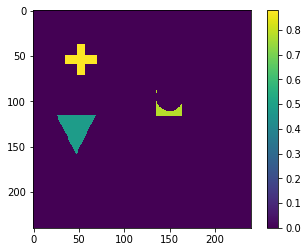
\includegraphics[width=\linewidth]{chapters/06_hdm/visualization/masked.png}
        \caption{Masked input image}
    \end{subfigure}%
    \begin{subfigure}{.33\textwidth}
        \centering
        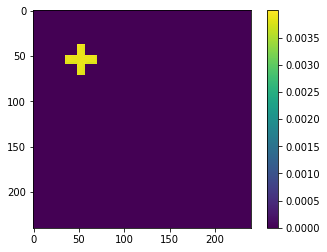
\includegraphics[width=\linewidth]{chapters/06_hdm/visualization/ground_truth.png}
        \caption{Baseline output segment from the unchanged image}
    \end{subfigure}
        \begin{subfigure}{.33\textwidth}
        \centering
        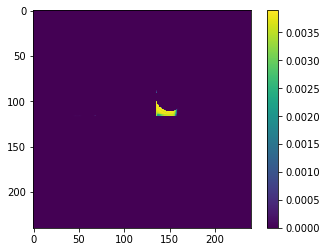
\includegraphics[width=\linewidth]{chapters/06_hdm/visualization/segment.png}
        \caption{Output segment from the masked image}
    \end{subfigure}
    \caption{The output segment (c) from the masked image (a) looks very different than the output segment from the unchanged image (b).}
    \label{hdm_visualization_sample}
\end{figure}

For visualization, a new blank image with the same size as the input image is generated. Next, we iterate over all the positions where masks have been
applied to input images. Each position has an associated Hausdorff distance which represents the distance of the output segment generated by the masked image and the baseline output segment.
At each position, we draw a circle with the same diameter as used when generating the mask. The color used to fill this circle represents the difference between the 

but this time we use a fill color which represents the difference of the Hausdorff distance 


\begin{figure}[H]
    \centering
    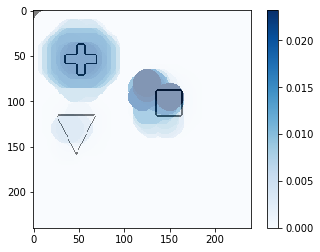
\includegraphics[width=8cm]{chapters/06_hdm/visualization/hdm_raw.png}
    \caption{Hausdorff distance between the left and the right figure: 1353. }
    \label{hdm_visualization_raw}
\end{figure}


\begin{figure}[H]
    \centering
    \begin{subfigure}{.5\textwidth}
        \centering
        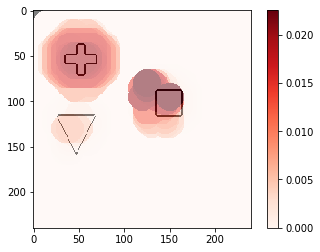
\includegraphics[width=\linewidth]{chapters/06_hdm/visualization/hdm_worse.png}
        \caption{Original shape}
    \end{subfigure}%
    \begin{subfigure}{.5\textwidth}
        \centering
        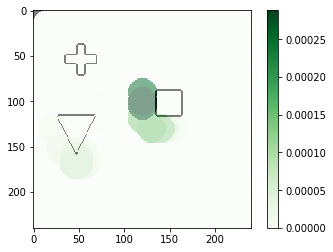
\includegraphics[width=\linewidth]{chapters/06_hdm/visualization/hdm_better.png}
        \caption{Shape moved to the right}
    \end{subfigure}
    \caption{Hausdorff distance between the left and the right figure: 1353. }
    \label{hdm_visualization_better_w}
\end{figure}
